\documentclass{article}
\usepackage{listings}
\usepackage{amsmath}
\usepackage{tabularx}
\usepackage{graphicx}
\usepackage{tikz}
\usetikzlibrary{shapes.geometric, arrows}
\usepackage{cite}
\usepackage{hyperref}
\usepackage{float}
\begin{document}
\lstset{language=python, tabsize=4}
\title{Node embedding}
\author{Yuchen Hou}
\maketitle

\section{Introduction}

\subsection{Deep learning in different domains}
\begin{itemize}
	\item image recognition
	\item speech recognition
	\item natural language processing
\end{itemize}

\subsection{Entity representations in different domains}

\subsubsection{Image representation: 2D light intensity array}
\begin{figure}[H]
	\centering
	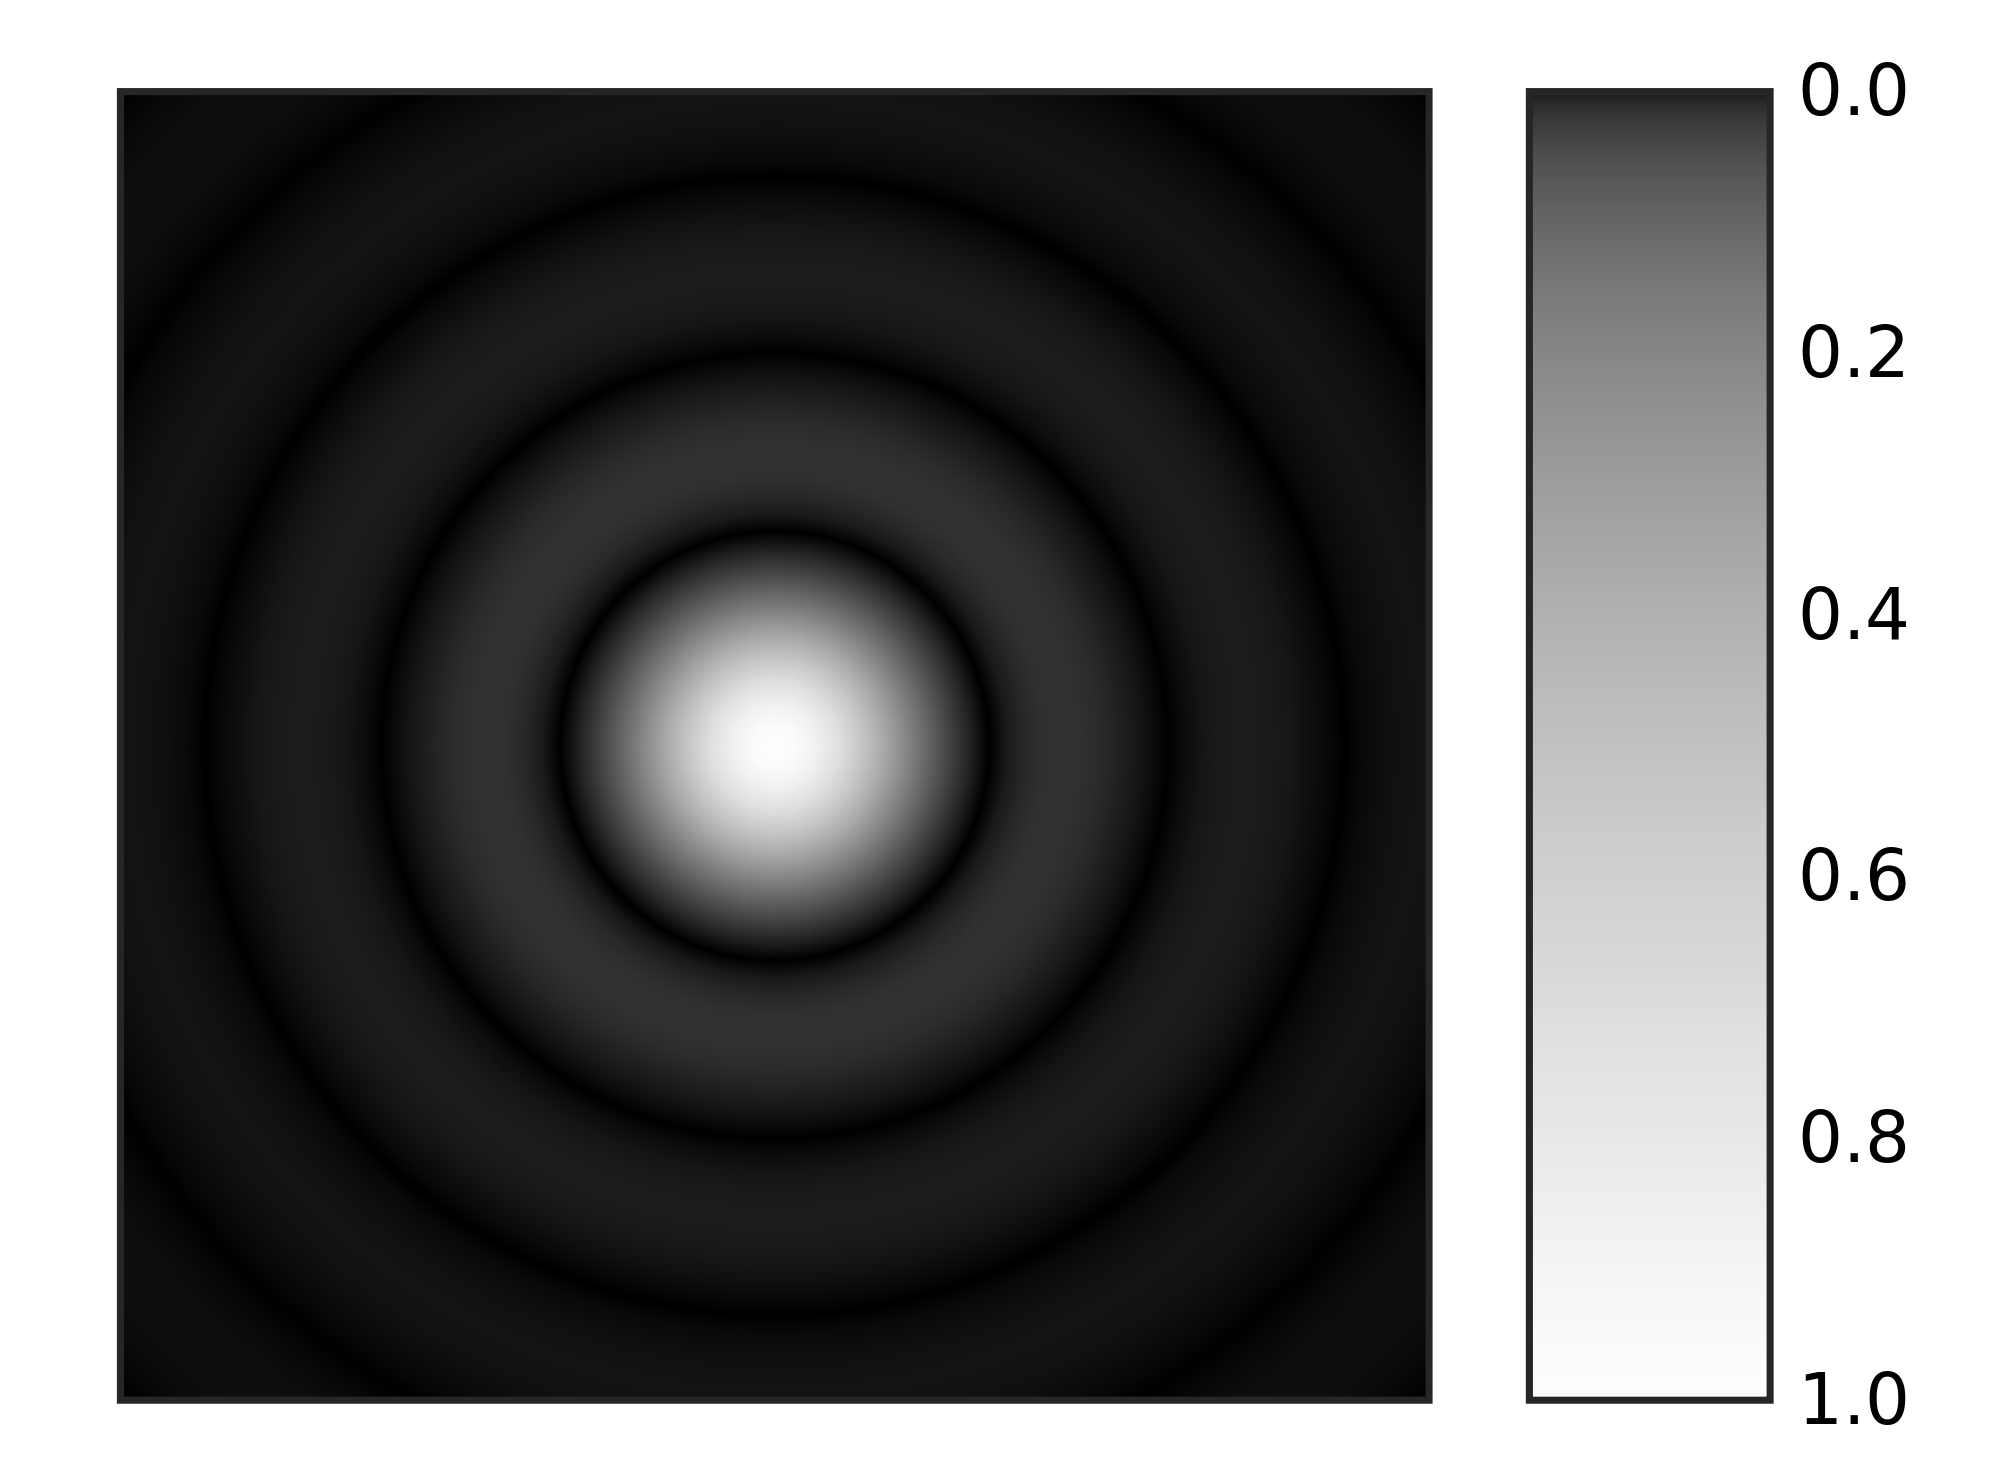
\includegraphics[width=0.5\linewidth]{Airy-pattern}
	\caption{\href{https://commons.wikimedia.org/wiki/File:Airy-pattern.svg}{the airy pattern} (John Doe / Wikimedia Commons / Public Domain): an image is represented by a 2D light intensity array.}
	\label{fig:Airy-pattern}
\end{figure}
\subsubsection{Utterance representation: 2D sound intensity array}
\begin{figure}[H]
	\centering
	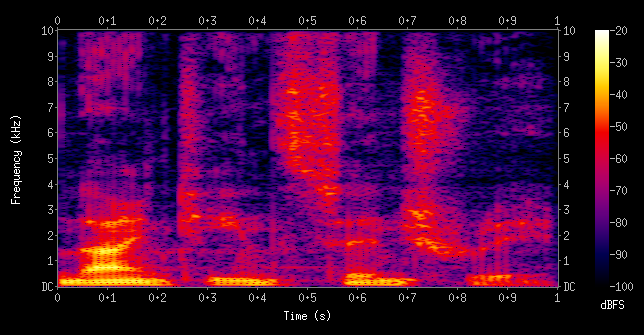
\includegraphics[width=\linewidth]{Spectrogram-19thC}
	\caption{\href{https://commons.wikimedia.org/wiki/File:Spectrogram-19thC.png}{Digitally produced spectrogram of a male voice saying [nineteenth century]}(Aquegg / Wikimedia Commons / Public Domain): a spectrogram is represented by a 2D sound intensity array.}
	\label{fig:Spectrogram-19thC}
\end{figure}
\subsubsection{Natural language representation: ?}
\begin{figure}[H]
	\centering
	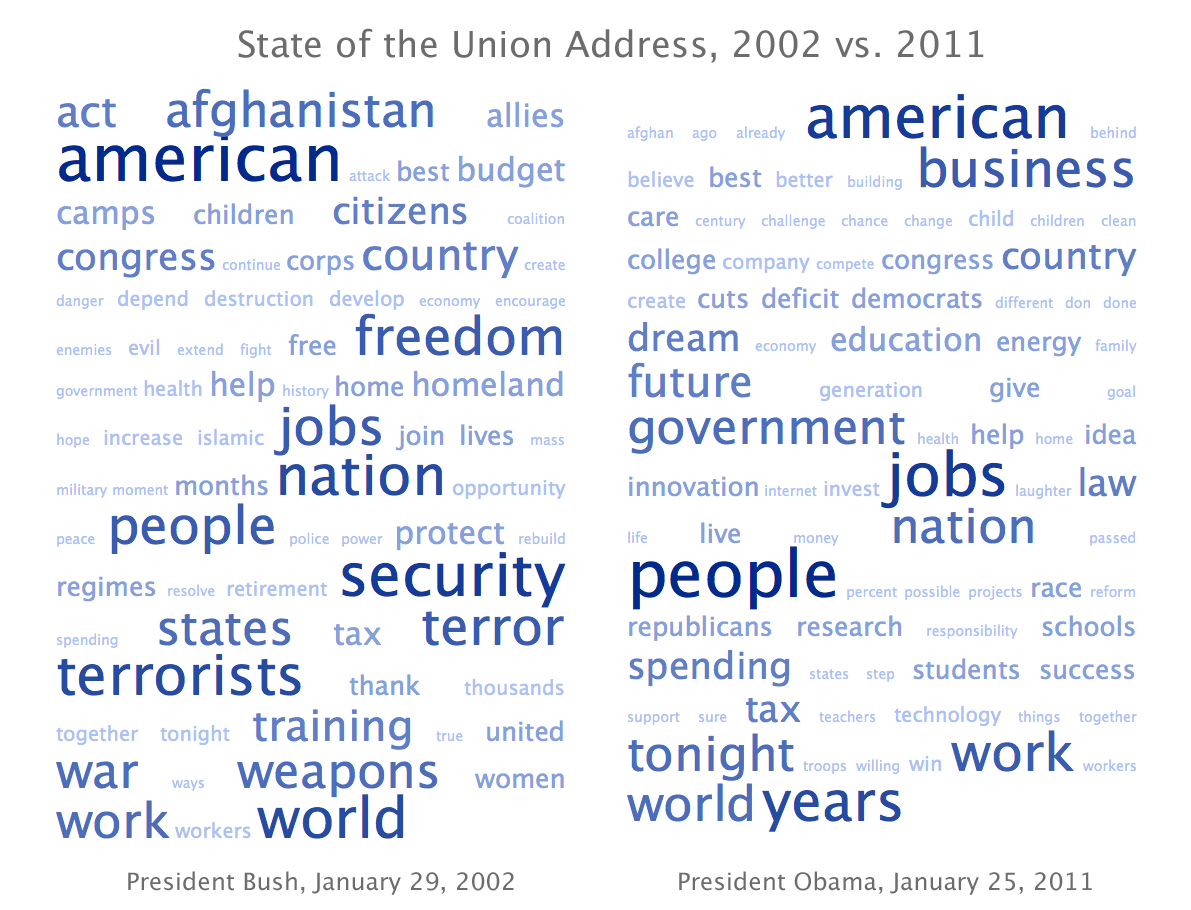
\includegraphics[width=\linewidth]{State_of_the_union_word_clouds}
	\caption{ \href{https://commons.wikimedia.org/wiki/File:State_of_the_union_word_clouds.png}{State of the union word clouds}(Pyrsmis / Wikimedia Commons / Attribution-Share Alike 3.0 Unported): words are conceptual.}
	\label{fig:State_of_the_union_word_clouds}
\end{figure}
\subsubsection{Graph representation: ?}
\begin{figure}[H]
	\centering
	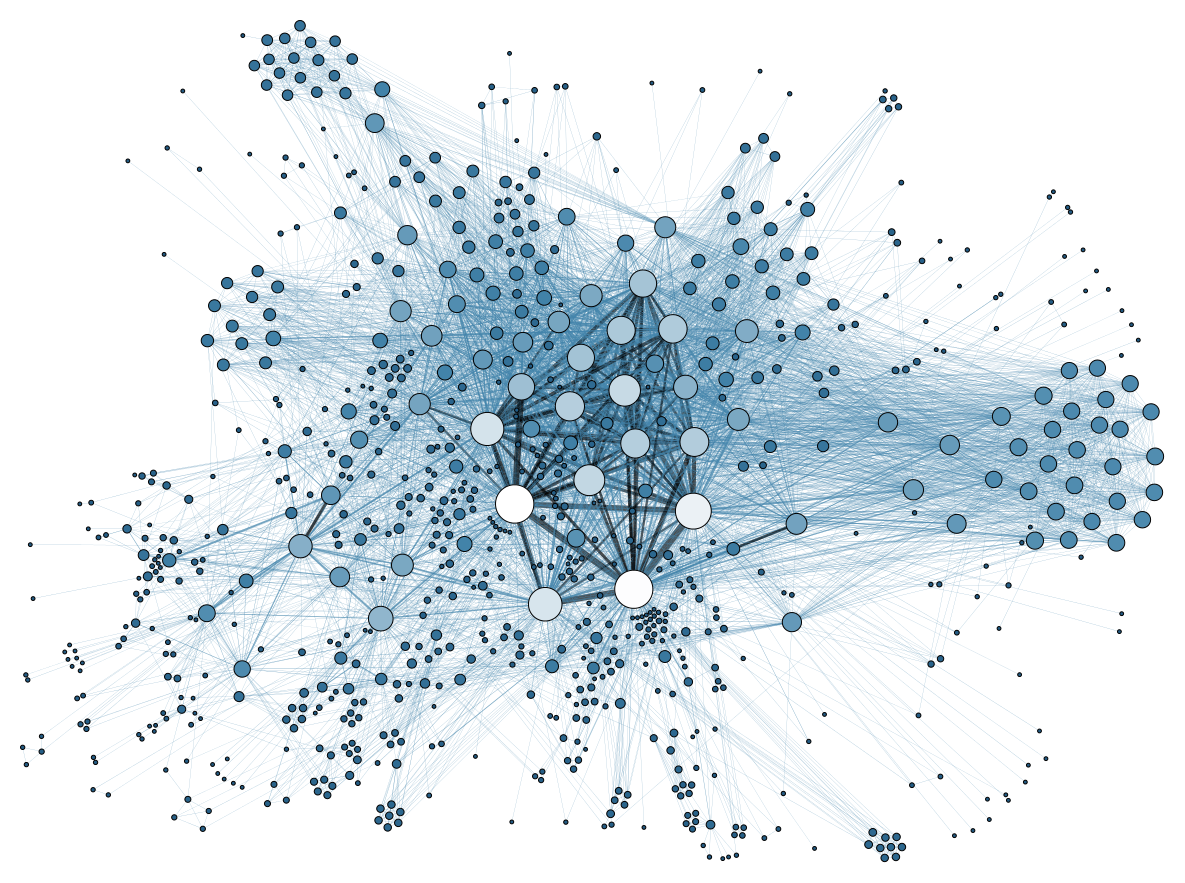
\includegraphics[width=\linewidth]{Social_Network_Analysis_Visualization}
	\caption{ \href{https://commons.wikimedia.org/wiki/File:Social_Network_Analysis_Visualization.png}{Social Network Analysis Visualization}(Martin Grandjean / Wikimedia Commons / Attribution-Share Alike 3.0 Unported): nodes are categorical.}
	\label{fig:Social_Network_Analysis_Visualization}
\end{figure}
\begin{itemize}
	\item light and sound intensities: measurable, numerical - easy for neural nets
	\item words, nodes and links: conceptual, categorical - hard for neural nets
	\item can we reduce words and nodes to numbers for neural nets?
\end{itemize}

\subsection{From natural language processing to graph mining}
\begin{itemize}
	\item word embedding: Mikolov 2013
	\item node embedding: Perozzi 2014
	\item node embedding for graphs with rich attributes: work in progress
\end{itemize}

\section{Word embedding}

\subsection{The goal}
\begin{itemize}
	\item represent words with meaningful numerical vectors for neural nets
\end{itemize}
\begin{table}[H]
	\centering
	\begin{tabularx}{\textwidth}{|X|X|X|} \hline
		rank & word & word vector \\ \hline
		1 & the & [2.309, 564, -9.5 ... 3] \\ \hline
		2 & be & [76, -342.2, 0.3 ... 4.1] \\ \hline
		3 & to & [-345, -834, 0.3 ... 34] \\ \hline
		... & ... & ... \\ \hline
		n & $ word_n $ & $ [x_1, x_2, x_3 ... x_d] $ \\ \hline
	\end{tabularx}
	\caption{Word vectors sorted by the popularity of the words in English: a word is represented by a vector of size d.}
	\label{tab:word}
\end{table}

\subsection{Observations and the approach}

\subsubsection{Sequence, word and context}
\begin{itemize}
	\item sequence = [guard, peace, and, justice, in, the, universe]
	\item word = [justice]
	\item context of radius 3 = [guard, peace, and, in, the, universe]
\end{itemize}
\subsubsection{Co-occurrences express relations and attributes}
\begin{table}[H]
	\centering
	\begin{tabularx}{\textwidth}{|c|X|c|} \hline
		co-occurrence & relation & attribute \\ \hline
		(guard, justice) & justice is protected because it's important and evil wants to destroy it & value, vulnerability \\ \hline
		(peace, justice) & justice is morally good and desirable, like peace & virtue \\ \hline
		... & ... & ... \\ \hline
	\end{tabularx}
	\caption{Attributes and relations about word [justice]: the information of a word is implicitly expressed by words in its contexts.}
	\label{tab:cooccurrences}
\end{table}
\subsubsection{Learn a word from its contexts}
\begin{itemize}
	\item learn [Jedi]: a member of the mystical knightly order in the Star Wars films, trained to guard peace and justice in the universe (Google Dictionary)
	\item learn every word supervised by the words in its contexts
\end{itemize}

\subsection{Implementation}

\subsubsection{Skip-gram model}\begin{figure}[H]
	\centering
	\newcommand{\layersep}{2.5cm}
	\newcommand{\vocabularySize}{8}
	\newcommand{\embeddingSize}{4}
	\begin{tikzpicture}[shorten >=1pt,->,draw=black!50, node distance=\layersep]
	\tikzstyle{every pin edge}=[<-,shorten <=1pt]
	\tikzstyle{neuron}=[circle,fill=black!25,minimum size=17pt,inner sep=0pt]
	\tikzstyle{input neuron}=[neuron, fill=green!50];
	\tikzstyle{output neuron}=[neuron, fill=red!50];
	\tikzstyle{hidden neuron}=[neuron, fill=blue!50];
	\tikzstyle{annot} = [text width=4em, text centered]
	
	% Draw the input layer
	\foreach \name / \y in {1,...,\vocabularySize}
	% This is the same as writing \foreach \name / \y in {1/1,2/2,3/3,4/4}
	\node[input neuron, pin=left:$ w_\y $] (I-\name) at (0,-\y) {};
	
	% Draw the hidden layer
	\foreach \name / \y in {1,...,\embeddingSize}
	\path[yshift=-2cm]
	node[hidden neuron] (H-\name) at (\layersep,-\y cm) {};
	
	% Draw the output layer
	\foreach \name / \y in {1,...,\vocabularySize}
	\node[output neuron, pin={[pin edge={->}]right:$ w_\y $}] (O-\name) at (2*\layersep,-\y) {};
	
	% Connect the input layer with the hidden layer
	\foreach \source in {1,...,\vocabularySize}
	\foreach \dest in {1,...,\embeddingSize}
	\path (I-\source) edge (H-\dest);
	
	% Connect the hidden layer with the output layer
	\foreach \source in {1,...,\embeddingSize}
	\foreach \dest in {1,...,\vocabularySize}
	\path (H-\source) edge (O-\dest);
	
	% Annotate the layers
	\node[annot,above of=H-2] {embedding layer};
	\node[annot,above of=I-2] {input layer};
	\node[annot,above of=O-2] {output layer};
	\end{tikzpicture}
	
	\caption{The skip-gram model with vocabulary size 8 and embedding size 4: learning a word vector supervised by its contexts}
	\label{fig:skipGram}
\end{figure}
\begin{itemize}
	\item linear units in the embedding layer: $ y_i = f(x_i) = w_i x_i $
	\item softmax units in the output layer: $ y_i = f_i(x) = \frac{exp(w_i \cdot x)}{\sum_{i = 1}^{n}exp(w_i \cdot x)} $
	\item cross entropy loss: $ loss = H(t, y) = - \sum_{i = 1}^{n} t_i log(y_i) $
\end{itemize}

\subsection{Learning outcome}
\begin{enumerate}
	\item word vectors stored in weights in embedding layer
	\item word vector distance $ \approx $ word semantic similarity
	\item word vector differences $ \approx $ word semantic relation
\end{enumerate}
\href{https://www.tensorflow.org/versions/r0.7/tutorials/word2vec/index.html}{word2vec visualization} by TensorFlow project

\section{Node embedding}

\subsection{The goal}
\begin{itemize}
	\item represent nodes with meaningful numerical vectors for neural nets
\end{itemize}
\begin{table}[H]
	\centering
	\begin{tabularx}{0.5\textwidth}{|c|c|X|} \hline
		ID & node & node vector \\ \hline
		1 & A & [2.3, 564, -9.5 ... 3] \\ \hline
		2 & B & [76, -342.2, 0.3 ... 4.2] \\ \hline
		3 & C & [-345, -834, 0.3 ... 34] \\ \hline
		... & ... & ... \\ \hline
		n & $ node_n $ & $ [x_1, x_2, x_3 ... x_d] $ \\ \hline
	\end{tabularx}
	\caption{Node vectors sorted by the node ID in a graph: each node is represented by a vector of size d.}
	\label{tab:node}
\end{table}

\subsection{Application scenario}

\subsubsection{The dataset}
\begin{table}[H]
	\centering
	\begin{tabularx}{0.5\textwidth}{|c|X| }  \hline
		nodeID & labels \\ \hline
		0 & [ture, false, false... true] \\ \hline
		1 & [ture, true, false... false] \\ \hline
		2 & [false, false, false... true] \\ \hline
		... & ... \\ \hline
		n & [ture, false, true... true] \\ \hline
	\end{tabularx}
	\caption{The node set: a node can have a number of labels.}
\end{table}
\begin{table}[H]
	\centering
	\begin{tabularx}{0.5\textwidth}{|X|X|}  \hline
		sourceID & destinationID \\ \hline
		0 & 4355 \\ \hline
		0 & 987876 \\ \hline
		2 & 324 \\ \hline
		... & ... \\ \hline
		n & x \\ \hline
	\end{tabularx}
	\caption{The link set: a link has no attributes}
\end{table}
\begin{itemize}
	\item dataset: graph = (nodes, links)
	\item link attribute: none
	\item node attribute: labels(list of booleans)
\end{itemize}

\subsubsection{Prediction task: node attribute prediction}
\begin{enumerate}
	\item input: X = node, node in nodes
	\item output: Y = [y[0], y[1], y[2] ... y[n-1]], y[i] in [true, false]
\end{enumerate}

\subsection{Observations and the approach}
\begin{table}[H]
	\centering
	\begin{tabularx}{\textwidth}{ |c|c|X| } \hline
		aspect  & natural language processing & graph mining \\ \hline
		dataset & corpus & graph \\ \hline
		basic entities & words & nodes \\ \hline
		entity collection & vocabulary & node set \\ \hline
		relations & co-occurrences (implicit) & links (explicit) \\ \hline
		entity sequences & sentences & random walks \\ \hline
		representation & word vector & node vector \\ \hline
	\end{tabularx}
	\caption{A comparison of natural language processing and graph mining from several aspects: from word embedding to node embedding.}
	\label{tab:wordVSnode}
\end{table}

\subsection{Implementation}

\subsubsection{Node embedding stage}
\begin{itemize}
	\item model: skip-gram model
	\item node sequence generation: sampled random walks on the graph
	\item weights update: weights in all layers
	\item learning outcome: node vectors stored in weights in embedding layer
\end{itemize}
\subsubsection{Label prediction stage}
\begin{itemize}
	\item model: adjust output layer size to label set size
	\item weights update: weights in output layer only
\end{itemize}
\begin{figure}[H]
	\centering
	\newcommand{\layersep}{2.5cm}
	\newcommand{\vocabularySize}{8}
	\newcommand{\embeddingSize}{4}
	\newcommand{\labelSetSize}{2}
	\begin{tikzpicture}[shorten >=1pt,->,draw=black!50, node distance=\layersep]
	\tikzstyle{every pin edge}=[<-,shorten <=1pt]
	\tikzstyle{neuron}=[circle,fill=black!25,minimum size=17pt,inner sep=0pt]
	\tikzstyle{input neuron}=[neuron, fill=green!50];
	\tikzstyle{output neuron}=[neuron, fill=red!50];
	\tikzstyle{hidden neuron}=[neuron, fill=blue!50];
	\tikzstyle{annot} = [text width=4em, text centered]
	
	% Draw the input layer
	\foreach \name / \y in {1,...,\vocabularySize}
	% This is the same as writing \foreach \name / \y in {1/1,2/2,3/3,4/4}
	\node[input neuron, pin=left:$ node_\y $] (I-\name) at (0,-\y) {};
	
	% Draw the hidden layer
	\foreach \name / \y in {1,...,\embeddingSize}
	\path[yshift=-2cm]
	node[hidden neuron] (H-\name) at (\layersep,-\y) {};
	
	% Draw the output layer
	\foreach \name / \y in {1,...,\labelSetSize}
	\node[output neuron, pin={[pin edge={->}]right:$ label_\y $}] (O-\name) at (2*\layersep,-\y-3) {};
	
	% Connect the input layer with the hidden layer
	\foreach \source in {1,...,\vocabularySize}
	\foreach \dest in {1,...,\embeddingSize}
	\path (I-\source) edge (H-\dest);
	
	% Connect the hidden layer with the output layer
	\foreach \source in {1,...,\embeddingSize}
	\foreach \dest in {1,...,\labelSetSize}
	\path (H-\source) edge (O-\dest);
	
	% Annotate the layers
	\node[annot,above of=H-2] {embedding layer};
	\node[annot,above of=I-2] {input layer};
	\node[annot,above of=O-2] {output layer};
	\end{tikzpicture}
	\caption{The label prediction model with node set size 8, embedding size 4 and label set size 2: learning label prediction.}
	\label{fig:label}
\end{figure}

\subsection{Strengths of this approach}

\subsubsection{Representing nodes as node vectors}
\begin{table}[H]
	\centering
	\begin{tabularx}{0.5\textwidth}{ |c|X|X| } \hline
		aspect  & node & link \\ \hline
		complexity & high & low \\ \hline
		observability & low & high \\ \hline
		example & user & activities \\ \hline
	\end{tabularx}
	\caption{A comparison of node and link with respect to their complexity and attribute observability: what one does tells us what kind of person he is.}
	\label{tab:nodesVSlinks}
\end{table}

\subsubsection{Online learning}
\begin{itemize}
	\item low memory requirement
	\item incremental model construction
	\item suitable for streaming graph
\end{itemize}

\subsection{Weaknesses of this approach}

\subsubsection{Node sequence generation}
\begin{enumerate}
	\item remote nodes in a deep walk is not strongly related to the root
	\item skip-gram's indifference to important node ordering
	\item power law node frequency distributions
\end{enumerate}

\subsubsection{Unable to use rich attributes in graph}
\begin{itemize}
	\item nodes and links have attributes
	\item attributes can provide more information than topology
\end{itemize}

\begin{figure}[H]
	\centering
	\newcommand{\layersep}{8}
	\newcommand{\vocabularySize}{3}
	\newcommand{\embeddingSize}{5}
	\begin{tikzpicture}[shorten >=1pt,->,draw=black!50, node distance=\layersep]
	\tikzstyle{every pin edge}=[<-,shorten <=1pt]
	\tikzstyle{neuron}=[circle, draw, minimum size=20]
	\tikzstyle{input neuron}=[neuron];
	\tikzstyle{output neuron}=[neuron];
	\tikzstyle{hidden neuron}=[neuron];
	\tikzstyle{annot} = [text width=4em, text centered]
	
	% Draw the input layer
	\foreach \name / \y in {1,...,\vocabularySize}
	\node[input neuron] (I-\name) at (0,-2*\y) {$ user_\name $};
	
	% Draw the hidden layer
	\foreach \name / \y in {1,...,\embeddingSize}
	\path[yshift=2cm]
	node[hidden neuron] (H-\name) at (\layersep,-2*\y) {$ movie_\name $};
	
	% Connect the input layer with the hidden layer
	\foreach \source in {1,...,\vocabularySize}
	\foreach \dest in {1,...,\embeddingSize}
	\path (I-\source) edge (H-\dest);
	\end{tikzpicture}
	
	\caption{The weakness of solely relying on topology and ignoring other rich attributes: unable to discriminate nodes.}
	\label{fig:weakness}
\end{figure}

\section{Node embedding for graphs with rich attributes}

\subsection{Advanced features/strengths}
\begin{enumerate}
	\item comprehensive learning: exploiting rich node and link attributes
	\item multi-task prediction: learn to predict any node or link attribute
\end{enumerate}

\subsection{Application scenario}

\subsubsection{The dataset}
\begin{table}[H]
	\centering
	\begin{tabularx}{0.5\textwidth}{|X|X| }  \hline
		userID & french \\ \hline
		0 & false \\ \hline
		1 & false \\ \hline
		2 & true \\ \hline
		... & ... \\ \hline
		n & false \\ \hline
	\end{tabularx}
	\caption{The node set: a user has 1 boolean attribute - french}
	\label{tab:user}
\end{table}
\begin{table}[H]
	\centering
	\begin{tabularx}{0.5\textwidth}{|X|X|X| }  \hline
		userID & movieID & rating \\ \hline
		0 & 4355 & 4 \\ \hline
		0 & 987876 & 7 \\ \hline
		2 & 324 & 2 \\ \hline
		... & ... & ... \\ \hline
		n & x & 9 \\ \hline
	\end{tabularx}
	\caption{The link set: a link has 1 numerical attribute - rating}
	\label{tab:rating}
\end{table}
\begin{itemize}
	\item dataset: graph = (\{users and movies\}, ratings)
	\item movie attribute: none
	\item user attribute: french(boolean)
	\item link attribute: rating(numerical)
\end{itemize}

\subsubsection{Prediction task: node attribute prediction}
\begin{enumerate}
	\item input: X = user, user in users
	\item output: Y = french, french in [true, false]
\end{enumerate}

\subsubsection{Prediction task: link attribute prediction}
\begin{enumerate}
	\item input: X = (user, movie), user in users, movie in movies
	\item output: Y = rating, rating in range(1, 10)
\end{enumerate}

\subsection{Observations and the approach}
\begin{enumerate}
	\item french: information about the user
	\item rating: information about the user and the movie
	\item learning: supervised by both attributes
\end{enumerate}

\subsection{Implementation}

\subsubsection{Multi-task model}
\begin{figure}[H]
	\centering
	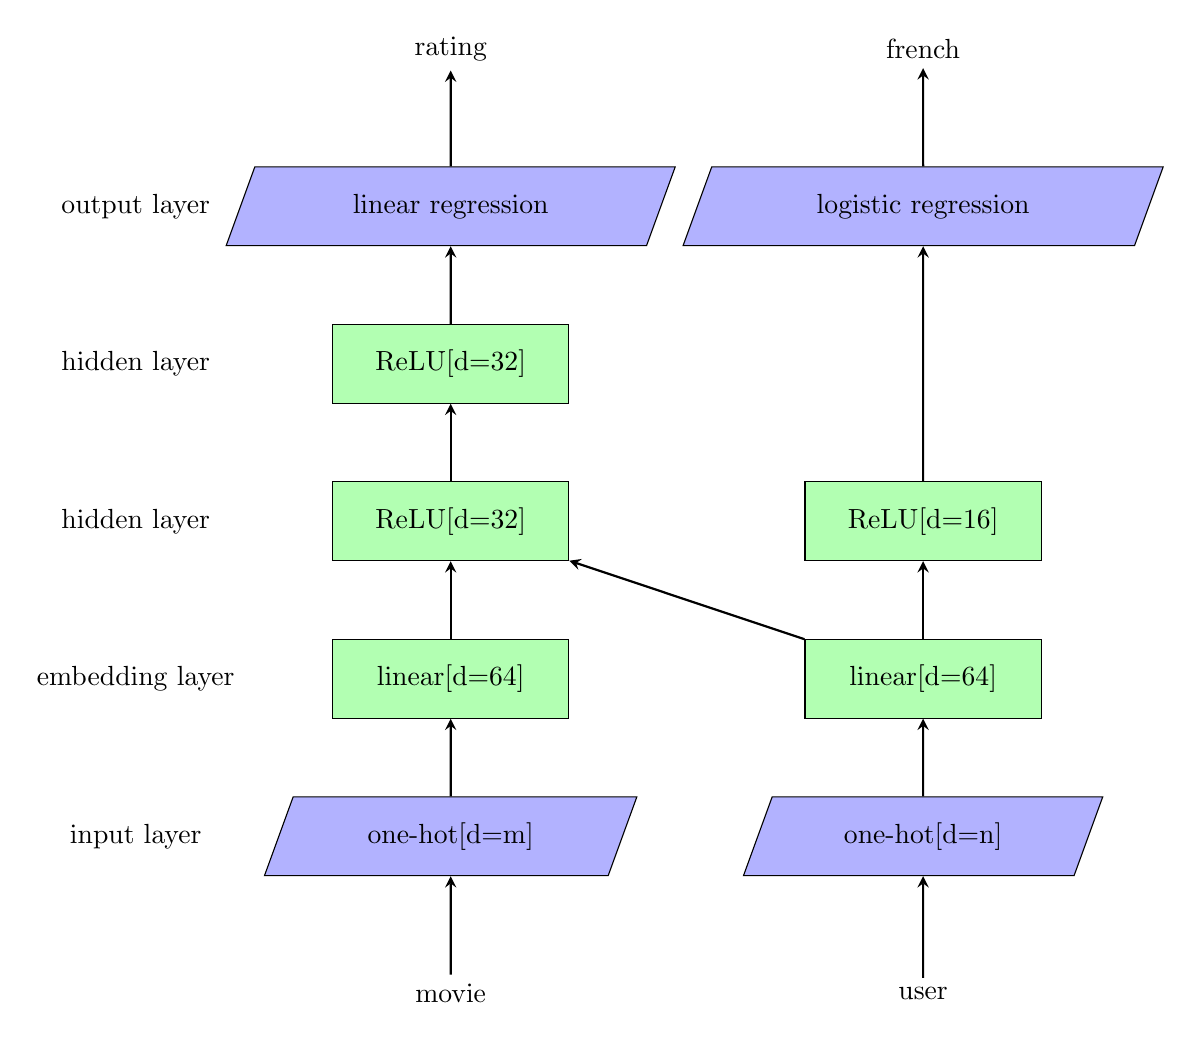
\begin{tikzpicture}[node distance=2cm]
	\tikzstyle{io} = [trapezium, trapezium left angle=70, trapezium right angle=110, minimum width=0cm, minimum height=1cm, text centered, draw=black, fill=blue!30]
	\tikzstyle{process} = [rectangle, minimum width=3cm, minimum height=1cm, text centered, draw=black, fill=green!30]
	\tikzstyle{arrow} = [thick,->,>=stealth]
	\node (linearRegression) [io] {linear regression};
	\node (logisticRegression) [io, right of=linearRegression, xshift=4cm] {logistic regression};
	\node (relu1) [process, below of=logisticRegression, yshift=-2cm] {ReLU[d=16]};
	\node (relu2) [process, below of=linearRegression] {ReLU[d=32]};
	\node (relu3) [process, below of=relu2] {ReLU[d=32]};
	\node (linear1) [process, below of=relu1] {linear[d=64]};
	\node (linear2) [process, below of=relu3] {linear[d=64]};
	\node (oneHot2) [io, below of=linear1] {one-hot[d=n]};
	\node (oneHot1) [io, below of=linear2] {one-hot[d=m]};
	\node (rating) [above of=linearRegression] {rating};
	\node (french) [above of=logisticRegression] {french};
	\node (output) [left of=linearRegression, xshift=-2cm] {output layer};
	\node (hidden2) [below of=output] {hidden layer};
	\node (hidden1) [below of=hidden2] {hidden layer};
	\node (embedding) [below of=hidden1] {embedding layer};
	\node (input) [below of=embedding] {input layer};
	\node (movie) [below of=oneHot1] {movie};
	\node (user) [below of=oneHot2] {user};
	\draw [arrow] (movie) -- (oneHot1);
	\draw [arrow] (user) -- (oneHot2);
	\draw [arrow] (oneHot2) -- (linear1);
	\draw [arrow] (oneHot1) -- (linear2);
	\draw [arrow] (linear1) -- (relu1);
	\draw [arrow] (linear1) -- (relu3);
	\draw [arrow] (linear2) -- (relu3);
	\draw [arrow] (relu3) -- (relu2);
	\draw [arrow] (relu1) -- (logisticRegression);
	\draw [arrow] (relu2) -- (linearRegression);
	\draw [arrow] (linearRegression) -- (rating);
	\draw [arrow] (logisticRegression) -- (french);
	\end{tikzpicture}	
	\caption{The multi-task prediction model with movie set size m, user set size n, embedding size 64: learning rating and french attribute prediction.}
	\label{fig:multiTask}
\end{figure}
\begin{itemize}
	\item embedding layer with linear units: $ y = f(x) = w x $
	\item hidden layers with ReLU(rectified linear units): $ y = f(x) = max(0, w x) $
	\item output layer with linear regression unit: $ y = f(x) = w x $
	\item output layer with logistic regression unit: $ y = f(x) = \frac{1}{1 + exp(-w x)} $
	\item hinge loss for logistic regression: $ loss = l(t, y) = max(0, 1 - ty) $
	\item squared error for linear regression: $ loss = l(t, y) = (t - y)^2 $
\end{itemize}

\section{Conclusions}
\begin{table}[H]
	\centering
	\begin{tabularx}{\textwidth}{ |c|c|c|X| }
		\hline domain & entity & representation & relations to other entities \\ 
		\hline image recognition & image & 2D array & NA \\ 
		\hline speech recognition & utterance & 2D array & NA \\ 
		\hline natural language & word & word vector & relations to other words \\ 
		\hline graph mining & movie & node vector & directed by director, etc \\ 
		\hline graph mining & user & node vector & rate movies, etc \\ 
		\hline graph mining & article & node vector & cite other articles, etc \\
		\hline
	\end{tabularx}
	\caption{A summary of various types of entities in different domains: numerical array representations for neural nets.}
	\label{tab:domains}
\end{table}
\begin{itemize}
	\item node embedding: neural net approach for learning vector representations of nodes
	\item online learning: good for streaming graph
	\item node embedding for graphs with rich attributes: low complexity, comprehensive learning and multi-task prediction
\end{itemize}
\begin{figure}[H]
	\centering
	
\includegraphics[width=\linewidth]{Thank-you-word-cloud}
	\caption{ \href{https://commons.wikimedia.org/wiki/File:Spectrogram-19thC.png}{Thank you word cloud}(Aquegg / Wikimedia Commons / Attribution-Share Alike 4.0 International)}
	\label{fig:Thank-you-word-cloud}
\end{figure}

\end{document}
